\documentclass[12pt,onecolumn]{article}
\usepackage[svgnames]{xcolor} % Enabling colors by their 'svgnames'
%%%%%%%%%%%%%%%%%%%%
% COMPILE WITH PDFLATEXMK
%%%%%%%%%%%%%%%%%%%%

%% PACKAGES
\usepackage{amsmath, amssymb}
\usepackage{graphics,graphicx}
\usepackage[colorlinks=false, linkcolor=red, citecolor=blue]{hyperref}
\usepackage{booktabs}
\usepackage{tikz}
\usepackage{framed}
\usepackage{float}
\usepackage{mathptmx}


\setlength{\parindent}{0pt}
\setlength{\parskip}{0.5em}

\usepackage{setspace}


\usepackage[font=footnotesize, labelfont={bf}]{caption}

\usepackage{authblk}
\renewcommand\Affilfont{\itshape\small}

%% USER DEFINED COMMANDS
\newcommand{\ellip}[1]{%
\begin{tikzpicture}[#1]%
\draw[rotate around={00:(0,0)}, shift={(0ex, 2ex)}] (0ex,0ex) ellipse (0.8ex and 0.3ex);
\end{tikzpicture}%
}

\newcommand{\rec}[1]{%
\begin{tikzpicture}[#1]%
\draw (0,0) rectangle (1.5ex, 0.6ex);
\end{tikzpicture}%
}

\newcommand{\dia}[1]{%
\begin{tikzpicture}[#1]%
\draw (0,0)   -- (0.8ex,0.3ex);
\draw (0.8ex,0.3ex) -- (1.6ex,0ex);
\draw (1.6ex,0ex) --(0.8ex,-0.3ex);
\draw (0.8ex,-0.3ex) --(0.0ex,0.0ex);
\end{tikzpicture}%
}

\newcommand{\ra}[1]{\renewcommand{\arraystretch}{#1}}

%\usepackage{lineno}
%\setlength\linenumbersep{8pt}
%\renewcommand\linenumberfont{\normalfont\tiny\sffamily\color{gray}}

\pagenumbering{gobble}
\usepackage[superscript,biblabel]{cite}



% HK commands

    \usepackage[paperwidth=9.5in,
    left=1in,
    right=1in,
    top=1in,
    bottom=1in,
    paperheight=11in,
    %margin=1in,
    footskip=.75in]{geometry}




    \usepackage{cmbright}
    \SetSymbolFont{largesymbols}{normal}{OMX}{iwona}{m}{n}


    %
    \usepackage[italic]{mathastext}
    %%% 'isomath' sets upper case greek letters italic in accordance with
    %%% the International Standard ISO 80000-2
    \usepackage{isomath}
    %



    % \definecolor{orange}{cmyk}{0,0.5,1,0}
    % \definecolor{HKblue}{cmyk}{65,4,0,0}
    % \definecolor{HKblue2}{cmyk}{100,0,0,0}


    \usepackage{comment}

    \setlength\marginparwidth{2.5in}
    \newcounter{commenthk}[section]
    \newenvironment{commenthk}[1][]{\refstepcounter{commenthk}\par\medskip
       \noindent\textbf{\thecommenthk.#1}
       %\rmfamily
       }{
       \medskip
       }


    \renewcommand{\comment}[2]{{\color{#1} $\blacksquare$ \footnote{\noindent \color{#1}#2} }}
    %\renewcommand{\c}[1]{{\color[magenta] $\blacksquare$ \footnote{\noindent \color[magenta]#1} }}

    \renewcommand{\c}[2][DarkGoldenrod]{{\color{#1}#2}}

    \newcommand{\commenti}[2]{{\scriptsize {\color{#1}\color{#1}(#2)} }}


    \renewcommand{\sl}[1]{\ensuremath{\textit{\textsf{\small #1}}}}

    \newcommand{\stone}[1]{ {\color{#1} \Large $\blacktriangleright$} }

    \newcommand{\commentm}[2][magenta]{{\color{#1}\marginpar
    {
        \color{#1}
            {
                \scriptsize\begin{commenthk}#2\end{commenthk}
            }
        }
    $^{\thecommenthk}$
     }}

    \newcommand{\commentf}[3]{{ \color{#1}
    \scriptsize
    \begin{commenthk}
    \parbox{#2}{#3}
    \end{commenthk}
    }
    %$^\thecommenthk$
     }
     \newcommand{\w}[1]{
     {\color[magenta]\uwave{\color{black} #1}}
     }
    \usepackage{ulem}
    \usepackage{showlabels}










\newcommand{\bs}[1]{\ensuremath{\boldsymbol{#1}}}

\newcommand{\mc}[1]{\ensuremath{\mathcal{#1}}}
\newcommand{\norm}[1]{\ensuremath \lVert #1 \rVert}
\newcommand{\GD}[1]{ D #1 (\boldsymbol{F})[\boldsymbol{H}]}
\newcommand{\GDI}[1]{ D #1 (\boldsymbol{I})[\boldsymbol{H}]}
\newcommand{\Lin}[1]{ L_{\boldsymbol{F}} #1 [\boldsymbol{H}]}
\newcommand{\LinI}[1]{ L_{\boldsymbol{I}} #1 [\boldsymbol{H}]}
%\newcommand{\Lin}[3][\boldsymbol{\varphi} ] {L_{\boldsymbol{#1}} #2 [#3]}
\newcommand{\Dm}[1]{\ensuremath{\boldsymbol{\varphi} } }



\renewcommand\thesection{\Roman{section}}
\renewcommand\thesubsection{\thesection.\arabic{subsection}}




\begin{document}







\paragraph{Cohesive zone (CZ) methods} have proven to be very significant for modeling interfacial fracture. There are several versions of CZ methods discussed in literature. Most of those methods can be put into two primary classes. The first class is roughly based on the numeric implementation of Hillerborg et al.\cite{hillerborg1976analysis}  while the second class is based on the ideas of Xu and Needleman~\cite{xu1994numerical}, and Camacho and Ortiz \cite{camacho1996computational}. Both classes are based on the work of Dugdale \cite{dugdale1960yielding} and Barenblatt \cite{barenblatt1962mathematical} and built atop of classical finite elements technqiues. In that crack growth is modeled by allowing adjoining finite  element pairs to separate along their shared boundary. As the elements seperate, tractions are applied on the separating faces of the elements as per a pre-assigned traction-separation law. The shape and parameters in the traction separation law are chosen to model different types of damage behavior (ductile, quasi-brittle, etc.). This idea is made numerically feasible by incorporating what are termed \textit{cohesive zone (or interface) elements} between the shared boundaries of adjoning finite element pairs. The primary difference beween the two classes of CZ methods is in the selection of the finite element boundaries at which the CZ elements are included.


In the classical version of the CZ method, given by Hillerborg et al., the CZ elements are only placed along finite element boundaries which are known\slash expected to be close to the final crack path. Thus, the application of the classical CZM is  predicated upon having some \textit{a priori} knowlege of the crack path. However, the success of the proposed research program hinges on developing and leveraging the ability to predict the evolution of complicated crack paths of which we have no or very little \textit{a priori knowledge}. Consequently, classical CZ methods are not suitable for the proposed research project.%ø


In the generalized version presented by Xu and Needleman the CZ elements are placed between all shared boundaries of the finite elements. This enables the simulation of crack propagation without requiring any \textit{a priori} knowledge of the crack path. This  generalized version is also capable of modeling the evolution of complicated crack paths. However, based on our study of the computational mechanics literature and the preliminary research that we undertook for planning the proposed project we found that the  generalized  CZ method is not very accurate in reproducing experimentally observed crack paths~\cite{tijssens2000numerical,de2003numerical,de2004computational}. For example,  Fig.~\ref{Fig:CZM} shows a comparison between   experimentally observed crack paths  and those that were computationally predicted using the generalized CZ method. As can be seen by comparing Fig.~\ref{Fig:CZM}(b) with either (c) or (d),  the generalized CZ method predicted cracks paths are quite different from the experimentally observed ones.  Furthermore,   as can be seen from  Figs.~\ref{Fig:CZM}(c)--(d), the generalized CZ method predicted crack paths are \textit{mesh dependent}. That is, they depend on the size and structure of the finite element mesh employed.



The inaccuracy and  mesh sensitivity of the generalized CZ method is widely discussed in literature \cite{de2003numerical,de2004computational,tijssens2000numerical,song2008comparative}.  For example, it is well known that  the crack path predicted by CZ method is inherently biased because crack growth in it is restricted to inter-finite element boundaries. This could give rise to mesh dependent crack paths. Also, Borst \cite{de2003numerical,de2004computational} gives the following reason for the method's poor performance. In theory, a CZ element is supposed to have infinite stiffness before the traction acting on it reaches a critical value, i.e, prior to initiation of any damage in it. In practice, however, in order to make the numerical implementation feasible, the CZ elements are provided with a finite stiffness  in the simulations. However, assigning a finite stiffness to the CZ elements can artifically change the bulk elastic constitutive behavior of the material composing the solid, since recall that the CZ elements are placed between all finite element boundaries in this method. This artifact can be avoided by increasing the CZ elements' stiffness. But that has the consequence of increasing the condition number of the numerical matrices in the simulation making the calculations unstable and prone to numerical errors. Borst suggests that this no win situation in selecting an ideal stiffness for the CZ elements coupled with the CZ elements being present between all shared finite element boundaries is the primary reason behind the method's poor performance.


We do not have any ideas as how to remedy the generalized CZ method's poor accuracy and high mesh sensitivity. Therefore, we decided not to select it for further development for the purpose of our pursing the project's overarching research objective.




\begin{figure}
    \centering
    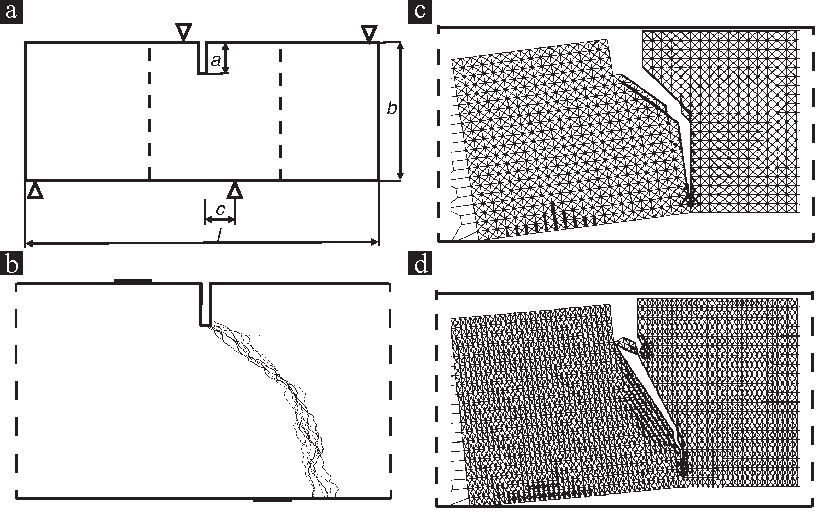
\includegraphics[width=1.0\textwidth]{./Figures/CZM/CZM_crack_path_ver2.pdf}
    \caption{
Comparison between experimentally observed and computationally predicted crack paths.
    (a) shows the set-up of the experiment, which is a single edge notch (SEN) shear load test.   (b) shows the experimental crack paths observed in concrete specimens by   Schlangen~\cite{schlangen1993experimental}. Each curve corresponds to a different specimen. (c) and (d) show the computationally predicted crack paths  for a coarse and fine finite  element mesh, respectively. These computational crack paths  were predicted by  Tijssens\textit{et al.}~\cite{tijssens2000numerical} for the experiments  shown in (a)--(b) using the generalized CZ method.}
    \label{Fig:CZM}
\end{figure}






\begin{figure}
    \centering
    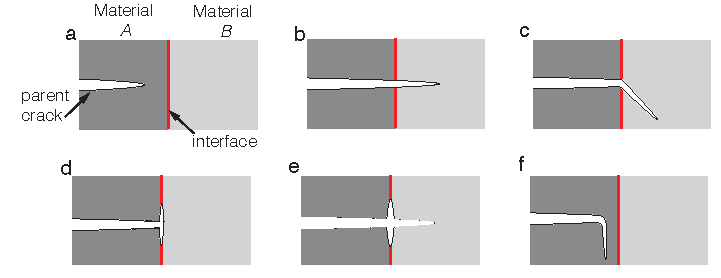
\includegraphics[width=1.0\textwidth]{./Figures/XFEM/CrackPathTopology.pdf}
    \caption{}
    \label{Fig:TopologyChanges}
\end{figure}




\paragraph{Extended Finite Element methods (XFEM).} The XFEM is a remarkable method. It has been used to  simulate quasi-static crack growth in both 2D~\cite{belytschko1999elastic,bordas2007extended,dolbow1999finite} and 3D~\cite{sukumar2000extended,moes2002non,gravouil2002non}, and dynamic crack growth in 2D~\cite{belytschko2003dynamic,song2006method}. It is currently widely used to predict crack paths~\cite{golewski2012numerical,barkai2012crack,peng2017extended} and is even a feature in the commercial finite element software package Abaqus~\cite{abaqus2014}.
It was introduced by Belytschko and Black \cite{belytschko1999elastic} for modeling cracks in solids without the need for remeshing. The numerical ideas underlying XFEM  are based on the partition of unity concept of Melenk and Babu\v ska~\cite{melenk1996partition}.  Currently, there are several versions of the XFEM  discussed in its literature. So, it is not unlikely that our comments will not apply to all of them. Also, we have sincerely tried not to cherry pick which features of the XFEM we discuss so as not to give an unfair appraisal of its capabilities.%ø




Like CZ methods, the XFEM too is built atop of finite elements methods. In  standard finite element method (FEM), the displacements, strains, etc. are approximated as  linear combinations of a select set of functions called  the \textit{basis functions}. Choosing a finite element mesh and the finite element type(s) (linear tetrahedron, etc.) in a problem  is tantamount to choosing the set of basis functions. In standard FEMs, the basis functions are usually continuous or smooth. The coefficients of the basis functions in the linear combinations are related to the degrees of feedom at the finite element nodes. In simulations based on  standard FEMs, the set of basis functions remains fixed during the simulations. The ingenuity of the XFEM lies in the following two modifications: (i) In addition to the usual continuous/smooth basis functions, discontinuous and irregular basis functions are allowed in the  set of basis functions. This process is called \textit{enrichment}. The choice of these discontinuous/irregular basis functions is  based  on the asymptotic solutions of fracture problems in the linear theory of elasticity and the total deformation theory of plasticity. These new basis functions enable the XFEM to capture the discontinuties across the crack's faces and the singular behavior  at its  tip. (ii) The  crack growth is modeled by allowing the set of basis functions to change as the crack grows.%ø


Despite its tremedous utility,  the XFEM is not suitable for pursuing the objectives of the current porposal.
This is  because  the XFEM in its classical form cannot  be used to  model topology changes (see, e.g., Fig.~\ref{Fig:TopologyChanges}). That is, it cannot  be used to capture phenomena such as  the merging of two (or more)  cracks to  form a single crack (Fig.~\ref{Fig:TopologyChanges}(a).i--ii), the splitting of a crack into two (or more)  daughter branches (Fig.~\ref{Fig:TopologyChanges}(b).i--iii), and  the nucleation of new cracks (Fig.~\ref{Fig:TopologyChanges}(c).i--iii).  This is not to say that XFEM cannot  apply to a crack that contains one of more branches. Indeed, special  enrichement functions have been developed through which  XFEM  can yield  the  displacements, stresses, etc.  in  problems that contain a crack with  multiple branches~\cite{daux2000arbitrary,belytschko2001arbitrary}. However, even  with those special enrichments  the XFEM  on its own---i.e., without any modeler input during the simulation, or \textit{a priori} knowledge about any  forthcoming topolology changes---will not be able to predict whether or not a  crack will split into mutiple branches, and if does split, how many branches it will split into.%ø


Topology changes are not very common in quasi-static crack growth problems in homogenous materials. However, as we discussed in \S XX,  topology changes are very common in heterogenous materials, such  as structural biomaterials. In fact,  topology changes are a key feature of the  mechanisms  through which  hypothesize that the structural biomaterials  gain their remarkable   toughness. It is possible to augument the XFEM with features from  CZ methods~\cite{wells2001new,moes2002extended,mariani2003extended}, or using older failure theories, such as the  \textit{critical principle stress failure criteria}, to give XFEMs some capability  for capturing toplology changes. However, we are not aware of any rational/scientific  theory that can guide such an augenmentation. Without a systematic means  to  guide the augumentation, we are afraid  that any such augementations can only be  hueristic or \textit{ad-hoc}  at best and therefore cannot be the primary agenda of a scientific project. The  RVF theory, on the other hand, can readily model topology  changes without any heuristic/\textit{ad-hoc} augumentations, see  Fig.~\ref{Fig:Concrete} and Fig.~\ref{second figure}, e.g.   For these reasons, we decided not to select the XFEM for  pursuing  the  project's research objective.
STOPPED HERE












% If the XFEM is
% that can  model the crack that constains one of more branches. What are saying is that given no \textit{a priori} information  about the potential topology . If it in



% The XFEM is directly applicable in its  classical form  to fracture experiments in which there are no topology changes as the  crack (resp. crack network)  grows (resp. evolves) .


% In collaboration with Prof. Sukumar's group at UCSD, we selected three such experiments and tried to predict the growth  (evolution) of the carck (crack patters) in those  experiments using the  XFEM method.    In all those  tests  we found that  the predictions of the XFEM to be indistinguisatble  from those we obtained from the   RVF theory. That is, both XFEM's and RVF theory's predictions were equally competiteive in reproducing the experimental observations. However, after careful consideration we decided not to use the XFEM method for pursuing the overarching objectives of this proposal since XFEM cannot readily capture topology changes.


% In its basic form,  XFEM method only yields the displacement, stress and other fields given a crack geometry. The XFEM is augemented with the  maximum hoop stress criteria to decide on the   direction in which the crack with growth  and with the Griffith's criteria to




% However, a number of issues arise by using enriched approximations~\cite{fries2010extended} and some of the critical ones
% are as follows:

% \begin{enumerate}
%     \item The employment of enrichment functions drastically decreases the accuracy of Gauss quadrature of the weak form. Even though many special quadrature approaches, e.g., decomposition of elements \cite{dolbow1999finite,belytschko2001arbitrary,sukumar2000extended,fries2008corrected}, adaptive integration~\cite{strouboulis2000design,strouboulis2000generalized,liu2004xfem,xiao2006improving} and integration by equivalent polynomials~\cite{iarve2003mesh,ventura2006elimination} are proposed to improve the accuracy of the quadrature, these approaches can be inefficient and time consuming.
%     \item The element matrices of the enriched elements can be ill-conditioned in some situations, e.g., when the ratio of the areas/volumes on both sides of the discontinuity is very large. The regular way to address this problem is to remove the enrichment of those nodes in the side of small supports ~\cite{daux2000arbitrary,liu2004xfem,bordas2007extended}.
%     \item The enrichment functions for crack tip, which are based on the knowledge of the analytical asymptotic solutions, are not always available or correct for complex fracture mechanics problems. One such example is that of a crack at the bimaterial interface, the crack tip displacement field based on LEFM is unphysical since the solution predicts that the crack faces interpenetrate near the crack tip~\cite{england1965crack}.
% \end{enumerate}


% \begin{figure}[t]
%     \centering
%     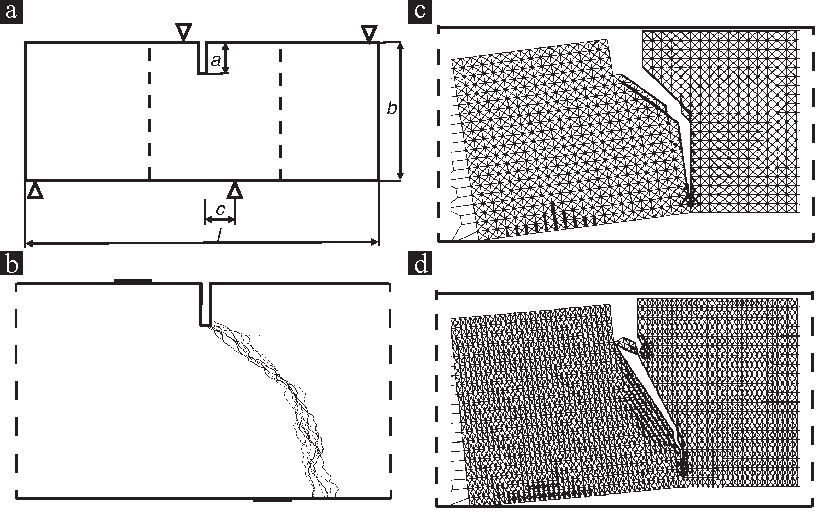
\includegraphics[width=1.0\textwidth]{./Figures/CZM/CZM_crack_path_ver2.pdf}
%     \caption{}
% \end{figure}










\begin{figure}[ht!]
    \centering
    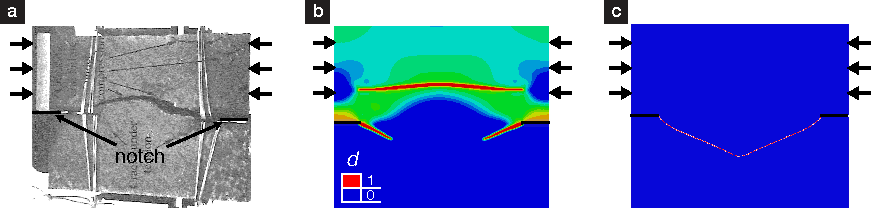
\includegraphics[width=0.75\textwidth]{./Figures/XFEM/concrete_ver2.pdf}
    \caption{Comparison between experimentally observed and computationally predicted crack paths.
(a) shows a photograph of a failed concrete specimen. This is from the expeiments reported by G{\'a}lvez \textit{et al.}~\cite{galvez1999fracture}.   The specimen was prepared by  cutting two notches, one  on each of its   left and righ edges.  The only loading on the specimen was on its  top portion. That is,   the region above the notches was loaded in compression. The specimen was observed to fail through the formation and  propagation of two distinct crack systems.  The first system   (marked in red dashed lines)  consists  of a two cracks, each of which  emanate  from a  notch and  grow a short distance into the  bottom portion of the specimen. The second system (marked in yellow dash-dot lines) consists  of a single crack that nucleates in the top portion of the speciemen and propagates symmetrically towards the left and right.  (b) shows the predictions of the RVF theory.  As can  seen, the    RVF theory captures both system 1 and 2 of the cracks formed. Its predicted shape and length of the  system 1 cracks is also quite consistent with what is experimentally observed.  Its  predicted shape and length of the system 2 crack is  slightly different from what is observed in experiments. We believe that this disparity is due to the incomplete knowledge we have about the specimen's materials properties and the experiment's loading program. (c) shows the predictions from the XFEM (as implemented in Abaqus). The XFEM method is able to capture the system 1 cracks. However, it completely misses the  system 2 cracks. This is expected, since as we discuss in the text, XFEM on its own cannot readily capture  toplogy changes, of which crack nucleation is a special case. Also, the XFEM predicted length of the  system 1 cracks is substantially  different from what is observed experimentally. }
    \label{Fig:Concrete}
\end{figure}















\newpage
\bibliographystyle{plain}
\bibliography{Mybib}

\end{document}
% Due to   (i) and (ii),  the same mesh can be used as the carck(s) grow.  That is there is no need for remeshing in XFEM. This feature is key to the XFEM's  tremendous popularity.


being able to  capture such phenamena is critical for achiving our research objective. Since,  as per our hypothesis, the tremendous enhancement in the toughness in composites with complex architectures involved the formation of a complex crack network, that is  precipitated by the e biomaterial's complex architectures.


The loading conditions along with formation of different crack patterns, before eventual failure of specimen obtained from \cite{galvez1999fracture} is shown in subfigure~(a) and the numerically predicted crack paths by RVFT and XFEM are shown in subfigures~(b) and (c), respectively.Red region in subfigure~(b) and (c), respectively, indicate the crack path. On comparing the subfigures~(a)-(c), we can see that RVFT qualitatively predicts the formation of a dominant crack in the region of compressive loading, whereas XFEM predicts a mode of failure which is inconsistent with the experimental results.

 The experimental results can be seen in Figure~\ref{Fig2}(b), where we see that  below the notches. However, these tensile cracks stop growing subsequently and the formation of a dominant crack in the compressive region occurs which eventually leads to failure. The crack paths from RVFT and XFEM are shown in Figures~\ref{Fig2}(b) and (c), respectively. RVFT qualitatively predicts the formation of short cracks in the tensile region and the formation of dominant crack in the compressive region. However, XFEM predicts that specimen will eventually fail by the extension of cracks in the tensile region which is inconsistent with the experimental results.
